\documentclass{article}
%\documentclass[journal]{IEEEtran}
%\documentclass{report}
%\documentclass{acta}

\usepackage{graphicx}
\usepackage{amsmath}


\begin{document}

\title{Introduction to the Perceptron and the application of pattern recogition techniques on real world problems}
\author{Peter Pollak, Stefan Sietzen, Albrecht V\"olkl}

\maketitle

\begin{abstract}
In the following article, we will discuss the application of the Perceptron to calculate the weight vector for a specific training set. We will also show an example of applying different pattern recognition techniques on a real world problem.
\end{abstract}


\section{Theory of the used techniques}

First we are going to explain what a Perceptron is and which pattern recogition techniques we have used in our research.

\subsection{Perceptron}

The perceptron was invented in 1957 by Frank Rosenblatt and is a type of a linear classifier, which means that it makes its predictions based on a linear predictor function combining a set of weights with the feature vector. 
\\The perceptron maps its input value \emph{x} to an output value \emph{f(x)} using the function
\\


\begin{equation}
f(x) = \begin{cases} 
    1, & \mbox{if } w \cdot x+b \mbox{ \textgreater \ 0} 
    \\ 
    0, & \mbox{otherwise }
\end{cases}
\end{equation}
\\

In this function, \emph{w} 	decribes a vector of real-valued weights, while $w \cdot x$ is the dot product, and \emph{b} is the constant \emph{\textbf{bias}} which is independent from any input value. Depending on whether the value of \emph{f(x)} is 0 or 1, x is classified either as a positive or negative instance,if we are dealing with a binary classificaton problem. If a negative value is chosen for \emph{b}, the weighted combination of inputs must provide a greater value than $|b|$ to be able to be able to reach a valoue over 0. In general, the bias alters the position of the decision boundary.
\\
A problem with the perceptron algorithm is that it won't terminate if if the learning set is not linearly seperable. If that is not the case, it is not possible to classify all vectors properly. A famous example for that problem is the \emph{Boolean Exclusive-Or problem}. 
\\
If the pereceptron is used in context of artifical neural networks, it is used an artificial neuron which is using the \emph{Heaviside step function} as the activation function. In combination with neural networks, one must also differ between a \textbf{single-layer-perceptron} and a \textbf{multi-layer-perceptron}. While a SLP consists of just a single layer of nodes in a directed graph, the MLP can work with several layers together.

\subsection{kNN Classifier}

The \emph{k-Nearest Neighbors Algorithm} is a non-parametric method which can be used for classification and regression. In our work, we have only experimented with the kNN algorithm as classifier. In this case, the output of the algorithm is a class membership where an object is classified by its neighbors. The new object checks which class is most common among it's $k$ nearest neighbors and is then assigned to that class. 

\subsection{Mahalanobis Distance}

The Mahalanobis Distance is a descriptive statistic that provides a relative measure of a data point's distance from a common point and was introduced by P.C. Mahalanobis in 1936. It can be defined in several ways, either by a distance of a multivariate vector $x$ from a group of values with mean $\mu$ and a covariance matrix $s$
\\
\begin{equation}
D_M(x) = \sqrt{(x-\mu)^TS^{-1}(x-\mu)}
\end{equation}
\\
or as a dissimilarity measure between two random vectors $\vec{x}$ and $\vec{y}$ of the same distribution with the covariance matrix S.

\begin{equation}
d(\vec{x},\vec{y}) = \sqrt{(\vec{x}-\vec{y})^TS^{-1}(\vec{x}-\vec{y})}
\end{equation}
\\
The Mahalanobis distance is mostly used in cluster analysis and classification techniques, for instance to detect outliers in the development of linear regression models, and was also widely used in biology.
\pagebreak

\section{Perceptron}

Implementing the preceptron, aside from the learnrate, doesn't leave much space for varation. Therefore it was no surprise, that our implementation had a 100 percent success rate applying it to the "perceptrondata" dataset with the target "perceptrontarget", which is a linearly sepearable combination. 

\begin{figure}
    \centering
    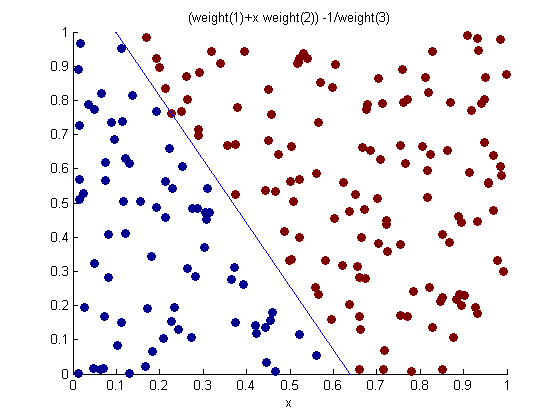
\includegraphics[width=3.0in]{200_of_200_correct}
    \caption{200 out of 200 correct}
    \label{200of200correct}
\end{figure}

The not linearly seperable "perceptrontarget2" had a success rate of 142/200, which is the maximum achievable with a linear discriminator.

\begin{figure}
    \centering
    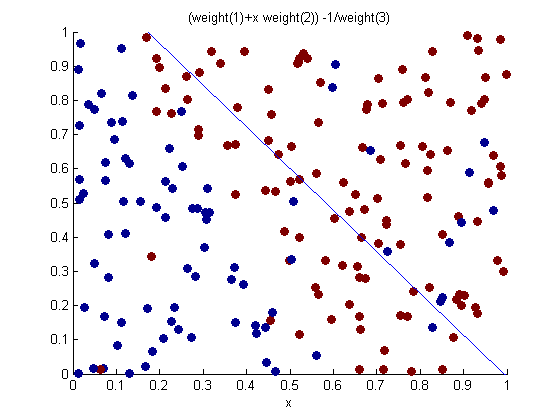
\includegraphics[width=3.0in]{142_of_200_correct}
    \caption{142 out of 200 correct}
    \label{142of200correct}
\end{figure}


The AND problem and the OR problem, which are obviously linearly seperable, where no problem for our perceptron function, while the XOR problem, as expected, didn't produce a valid result

\begin{figure}
    \centering
    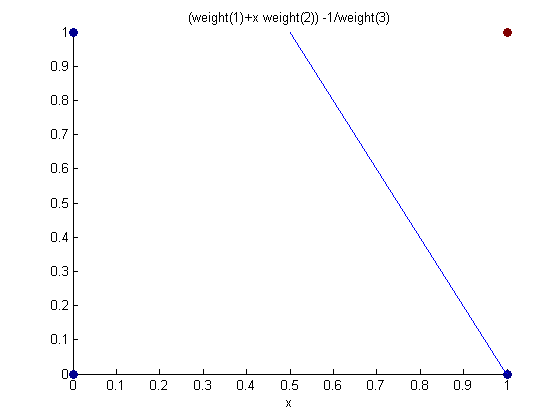
\includegraphics[width=3.0in]{and_correct}
    \caption{AND problem}
    \label{andproblem}
\end{figure}

\begin{figure}
    \centering
    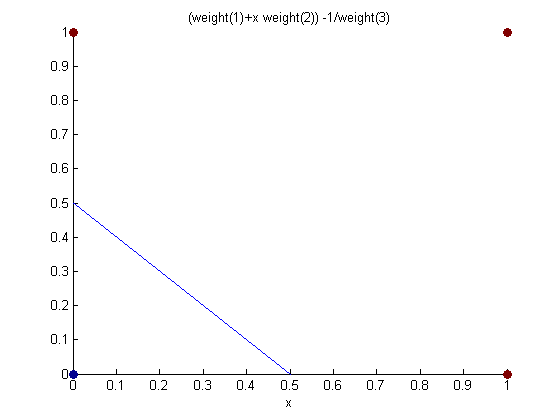
\includegraphics[width=3.0in]{or_correct}
    \caption{OR problem}
    \label{orproblem}
\end{figure}

\begin{figure}
    \centering
    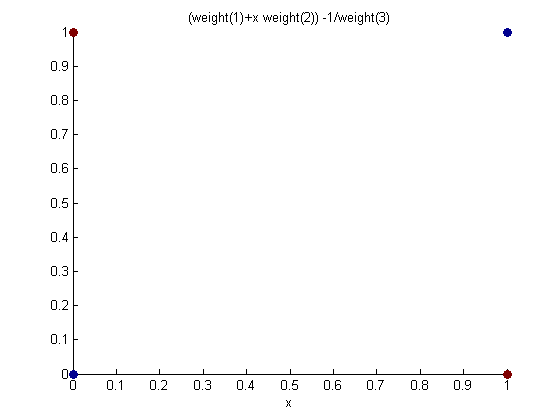
\includegraphics[width=3.0in]{xor_wtf}
    \caption{XOR problem}
    \label{xorproblem}
\end{figure}


\section{Practical Application}

When applying the 3 different classificators to a real world problem, we noticed, that our kNN algorithm outperformed the perceptron and the mahalanobis classificators. 

\subsection{Perceptron}

The problem with the perceptron in this case are the 6 different classes, which the perceptron is not suited for. We therefore used the perceptron to just classify between the dry and the wet strokes, where it had an acceptable success rate of around 80 percent. By reducing the feautures, we could achieve a successs rate of 86 percent.

\begin{figure}
    \centering
    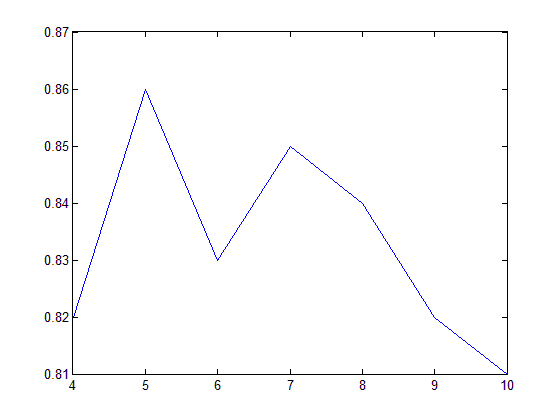
\includegraphics[width=3.0in]{perceptron_feature_number_successrate}
    \caption{Perceptron Feature Number Successrate}
    \label{perceptron}
\end{figure}

We therefore assume, that the stroke classification is not perfectly solvable with a linear discriminator, like the combination of "perceptrondata" and "percenptrontarget2", where there was only a success rate of 142/200 compared to the linearly discriminable "perceptrontarget", where the successrate of our perceptron implementation was 100 percent.

\subsection{kNN Classifier}

The kNN on the other hand, despite it simplicity performed really well, already giving 51 percent correct results at k=1, going to 87 percent correct results with k=6

\begin{figure}
    \centering
    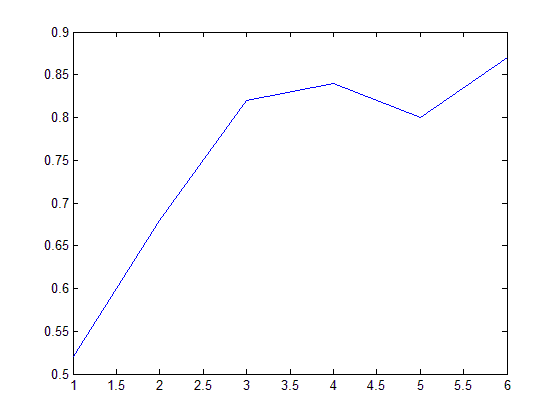
\includegraphics[width=3.0in]{kNN_graph}
    \caption{kNN graph}
    \label{knngraph}
\end{figure}

Also note that different feature sets gave different results. When initially using all 20 features for classification, we got a success rate of 82 percent, by selecting the best features we could raise that percentage to 87 percent with k=6. We did that by first selecting the best performing single feature set and then successively always the best combination with one more feature. We found that a combination of 7 features gave us good results.

\subsection{Mahalanobis Distance0}

The mahalanobis distance classificicator was really disappointing in this application, it only achieved a success rate of 9/77 correct classifications applied to the stroke problem. we didn't find out why this was the case, but we assume that it could be tweaked by selecting a beter featureset. The complexity and high dimensionaliaty of this classification problem is apparently not suited to apply a mahalanobis-distance classificator rather naively to.

\section{Comparison of the Perceptron and Pattern Recognition Algorithms}

Conclusively the kNN algorithm was best suited for the application with the stroke images, as it produced good results even before feature reduction. The perceptron is really limited in its application, due to its binary nature. It did perform well on discriminating dry and wet strokes though. The mahalanobis was not suited very well to applying it without feature reduction in this problem, even when reducing the features it didn't improve near to an acceptable sucess rate.


\end{document}